\chapter{Asymmetrical Conductor with a Hole \\ TEAM Workshop Problem 7}

\modinfo{Directory}{TEAM7}
\modinfo{Solvers}{\Idx{CoilSolver}, \Idx{WhitneyAVSolver},\Idx{MagnetoDynamicsCalcFields}}
\modinfo{Tools}{\Idx{ElmerGUI}}
\modinfo{Dimensions}{3D, Transient}
\modinfo{Author}{Jonathan Velasco}


\subsection*{Case definition}

The Testing Electromagnetic Analysis Methods (TEAM) Problem 7 is a validation case consisting of a thick aluminium plate with a hole,  which is placed eccentrically in a non-uniform magnetic field.  The field is produced by a sinusoidal current flowing through a coil that hovers over the plate as shown in Fig. \ref{fg:geometry} .  Due to asymmetry a simplification of the model becomes unavailable and a full 3D model is needed.   The goal of the model is to demonstrate the basic setup of a 3D eddy current problem.

\begin{figure}[H]
\centering
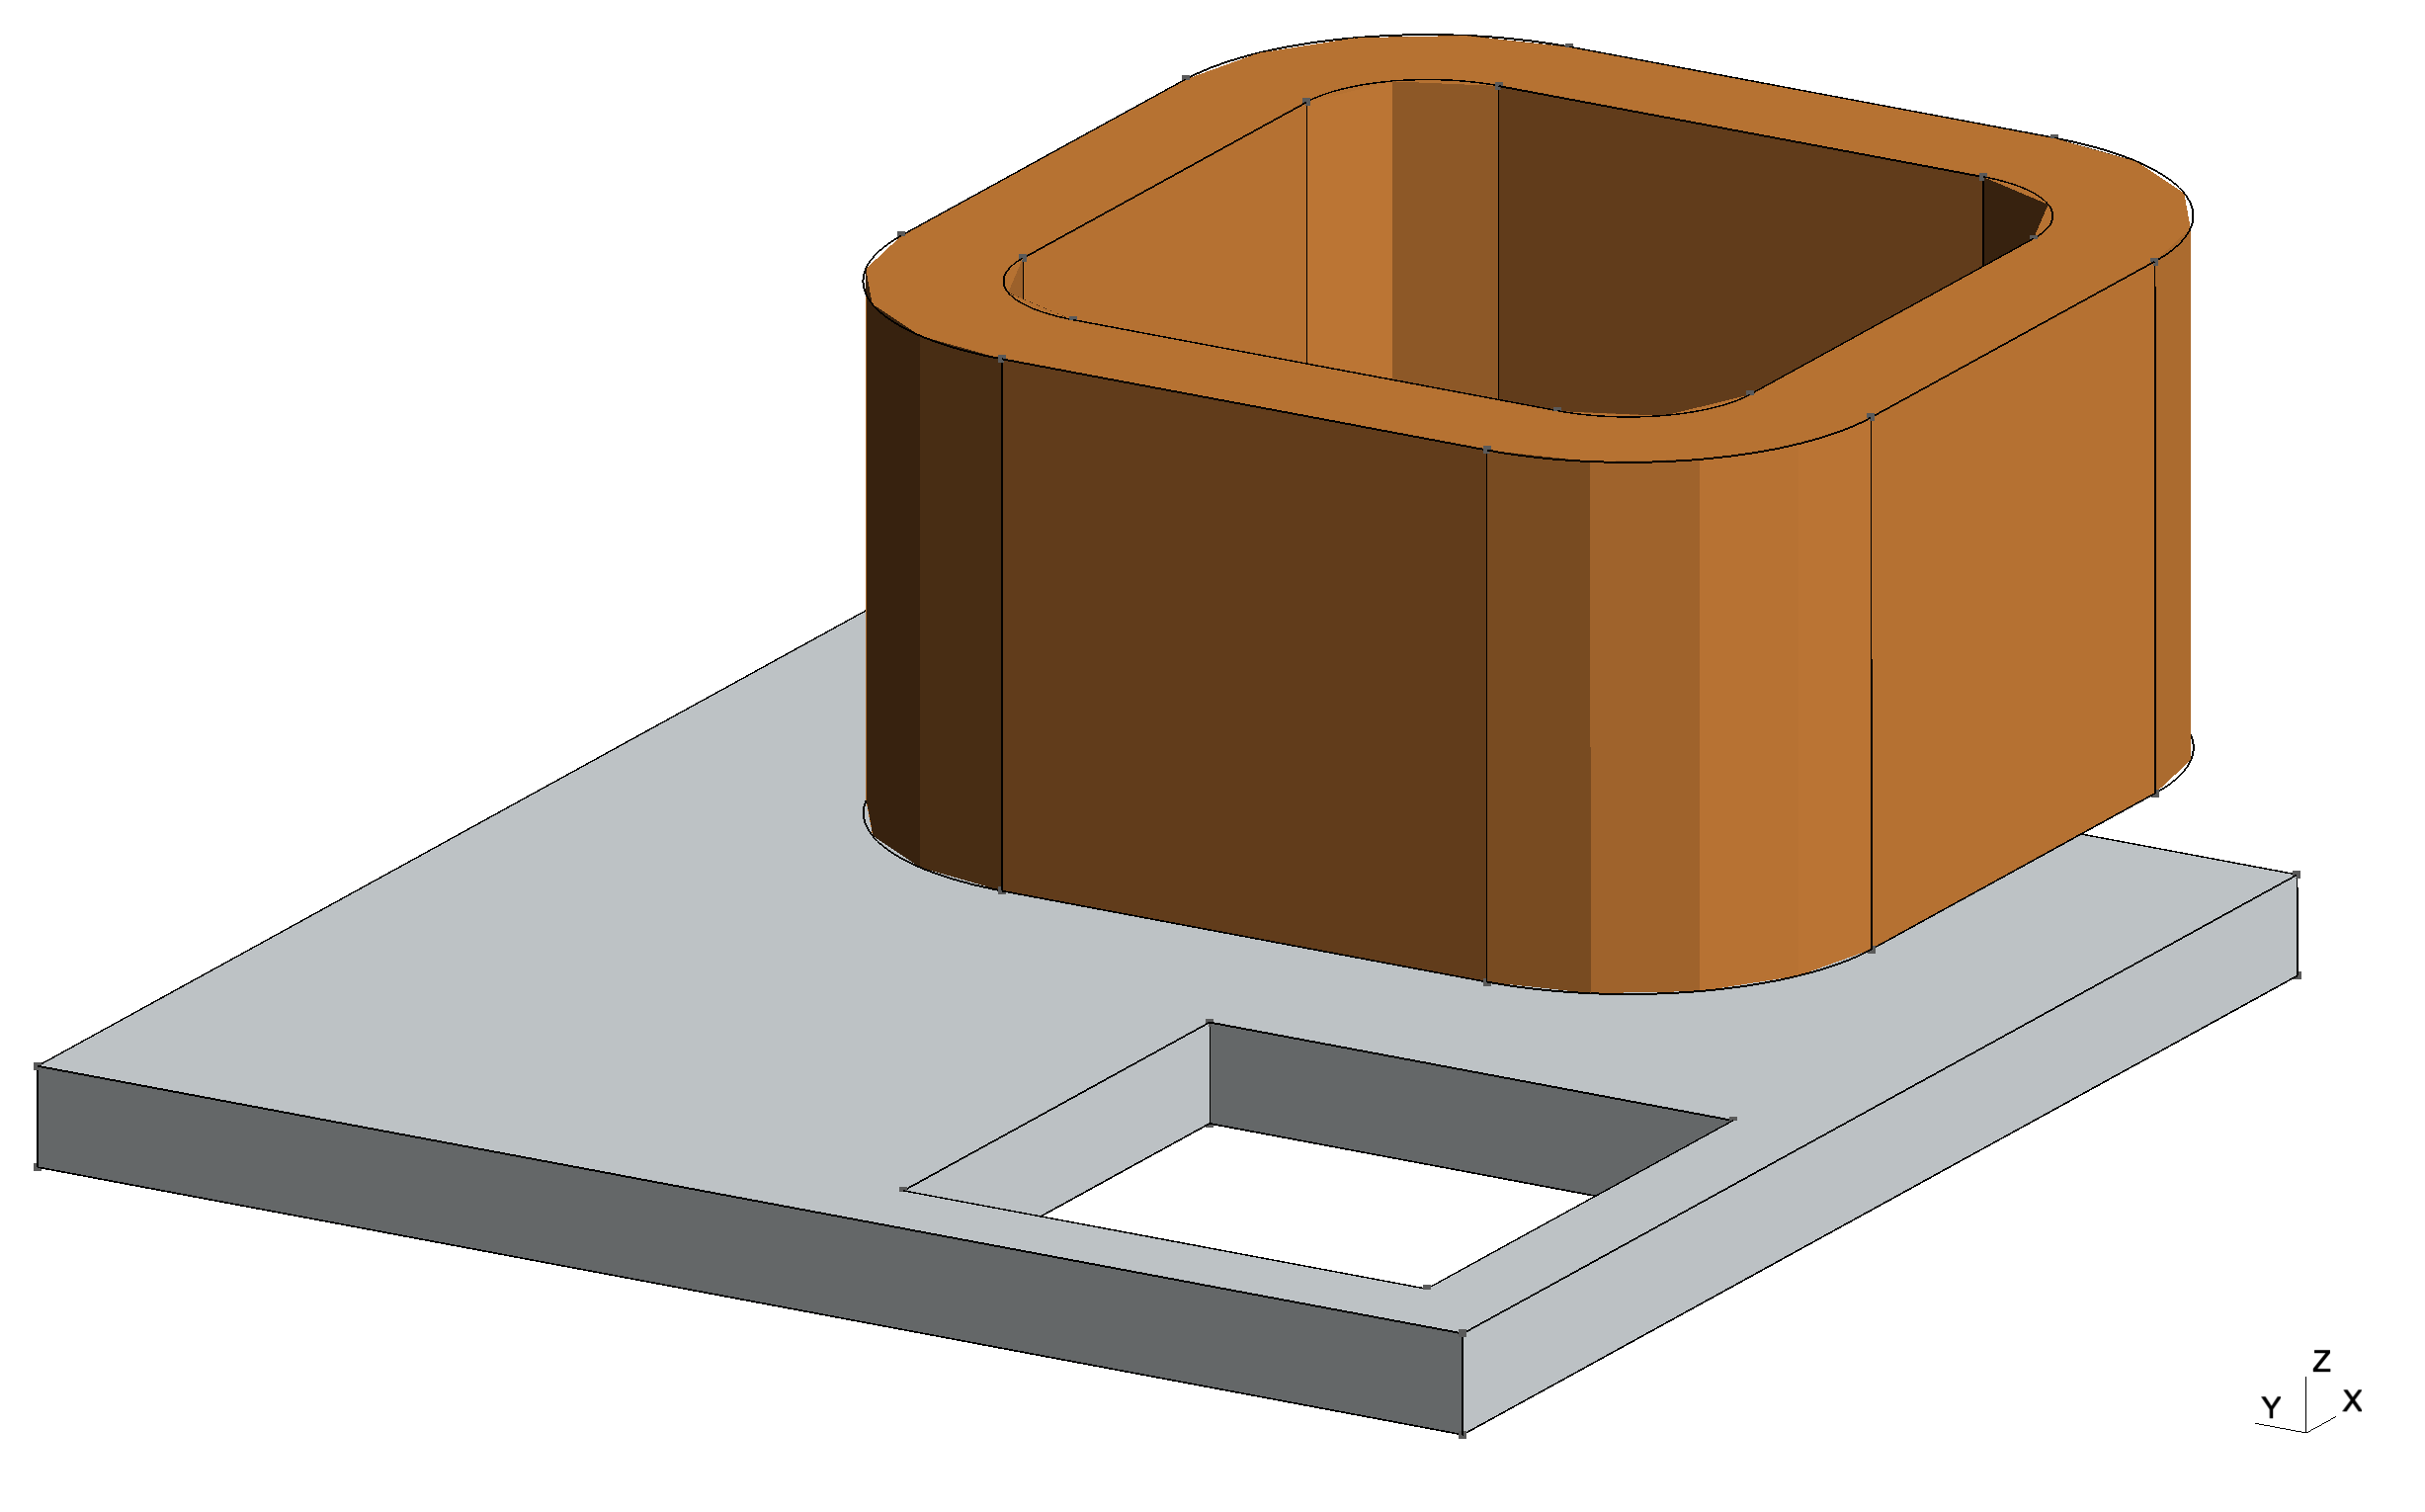
\includegraphics[width=0.6\textwidth]{figures/TEAM7_geo.png}
\caption{TEAM Problem 7 Geometry Description}\label{fg:geometry}
\end{figure}  

\noindent The full description of the given problem can be found in the COMPUMAG website under: \\
 \href{https://www.compumag.org/wp/wp-content/uploads/2018/06/problem7.pdf}{\textbf{TEAM Problem 7}} 
 
\noindent Mesh and tailored .sif file can be found in our Github repository under the TEAM7 directory: \\
 \href{https://github.com/ElmerCSC/elmer-elmag}{\textbf{Elmer Electromagnetics Tutorials}}  
 
 \clearpage
 \subsection*{Meshing: From Gmsh to ElmerGrid} 
 
 The TEAM7 Mesh can be found in our Github repository under the TEAM7 directory: \\
 \href{https://github.com/ElmerCSC/elmer-elmag}{\textbf{Elmer Electromagnetics Tutorials}}  \\
 
 \noindent However,  you may also want to import your own mesh from another software.  Under the same GitHub repository you'll find the .geo file created in Gmsh (gmsh/TEAM7.geo).  Note,  this mesh is generated with \href{http://gmsh.info}{Gmsh} but ElmerGrid parses several formats into ElmerSolver format. (e.g., .ansys, .inp, .fil, .mphtxt ...). \\
 
\noindent To mesh .geo file please run the following cmd/terminal command

\begin{verbatim}
gmsh TEAM7.geo -3
\end{verbatim}

\noindent where the $-$3 implies 3D meshing. This will save the mesh as TEAM7.msh

\noindent If further mesh refinement is needed:

\begin{verbatim}
gmsh TEAM7.msh -refine
\end{verbatim}

\noindent The command performs uniform mesh refinement. You can also perform barycentric refinement with command: $-$barycentric$\_$refine. \\
 
\noindent Once the mesh is saved you can parse it into ElmerSolver by using the following command

\begin{verbatim}
ElmerGrid 14 2 TEAM7.msh
\end{verbatim}

\noindent where 14 denotes the input mesh format (Gmsh) and 2 the output mesh format (ElmerSolver).  

\noindent The mesh is ready to be used by ElmerSolver either using command line or ElmerGUI.
 
 
 
\subsection*{Necessary Solver Modules} 
 
The TEAM7 magnetodynamics problem can be solved using two modules: the \textit{Coil Current Solver} and the \textit{WhitneyAVSolver}.  The field solution can be retrieved using the \textit{MagnetoDynamicsCalcFields} module.\\

The \textit{Coil Current Solver} solves for the irrotational electric field associated with the gradient of the electric scalar potential.  Hence,  the current density is calculated and may be used as an external source (Body Force) when solving the magnetodynamics problem.  The magnetodynamics problem is then solved throughout the whole domain (coil,  plate and air) using the  \textit{WhitneyAVSolver} and the field solution such as the magnetic flux density,  magnetic field strength among other variables can be obtained for postprocessing visualization using the \textit{MagnetoDynamicsCalcFields} module.



\subsection*{ElmerGUI Project}

Start \texttt{ElmerGUI} from command line or by clicking the icon in your desktop. Here we describe the essential steps in the \texttt{ElmerGUI} by writing out the click-by-click procedure.  Indentation generally means that the selections are done within the window chosen at the higher level. 

Before setting up the model,  let us configure \texttt{ElmerGUI}'s menu and necessary settings related to this particular model by using the top ribbon in the GUI (Fig. \ref{fg:ribbon})

\begin{figure}[H]
\centering

\includegraphics[width=0.7\textwidth]{figures/ribbon.png}
\caption{Top Menu}\label{fg:ribbon}
\end{figure}  

For simplicity the project directory is presented under ElmerGUI$\_$TEAM7. The model is solved using modules \textit{Coil Current Solver}, \textit{WhitneyAVSolver} and \textit{MagnetoDynamicsCalcFields},  which are found under the \textit{coilsolver.xml} and \textit{magnetodynamics.xml} menus.  As of the current version of the code,  these menus are not added automatically and need to be added manually.   Let us setup the project directory,  load the mesh (TEAM7) in ElmerSolver format (.mesh.*) and load the necessary menus.  See Fig 



\begin{verbatim}
File
  New project ...
      Project directory 
          Select project dir -> ElmerGUI_TEAM7
      Geometry input
          Elmer mesh -> TEAM7
      Extra EDFs to be added
          Add -> coilsolver.xml
          Add -> magnetodynamics.xml
  OK
\end{verbatim}


\begin{figure}[H]
\centering
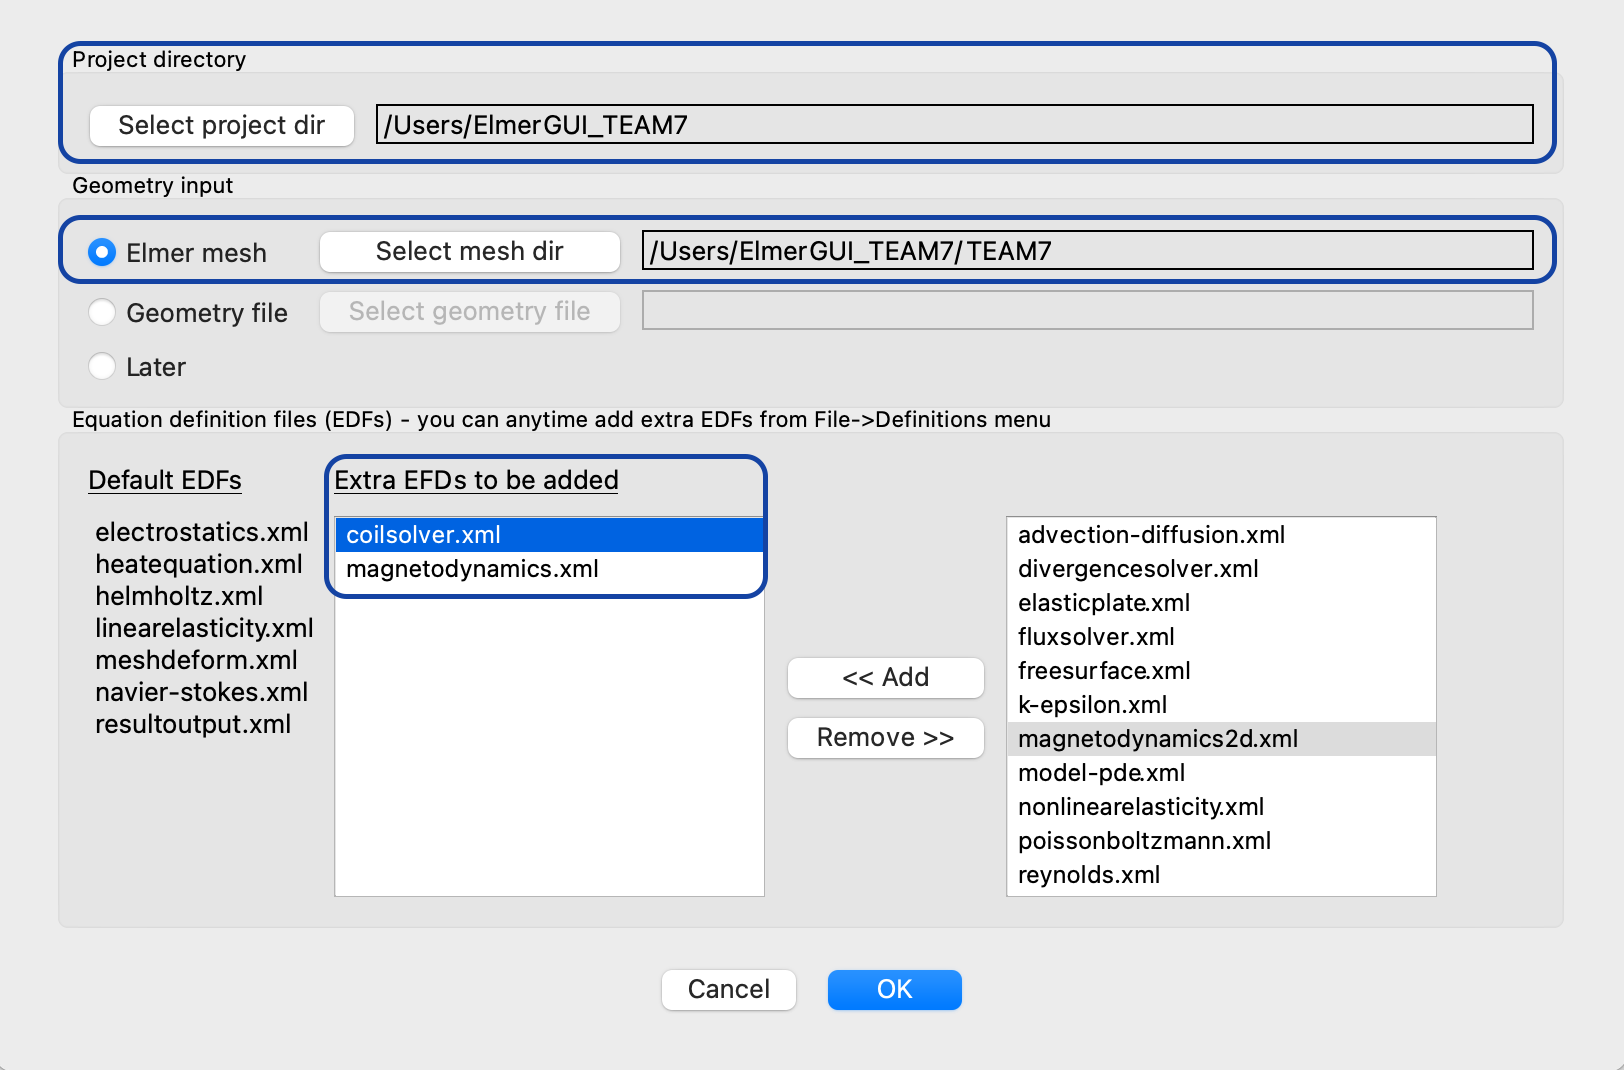
\includegraphics[width=0.7\textwidth]{figures/new_project.png}
\caption{New Project Window}\label{fg:new_project}
\end{figure}  


Adding additional menus can be avoided by permanently moving the .xml files from \texttt{\$ELMER\_HOME/install/share/ElmerGUI/edf-extra} to \texttt{\$ELMER\_HOME/install/share/ElmerGUI/edf}\\


\subsection*{Model Preferences}

The TEAM Problem 7 is solved by imposing a transient sinusoidal current that generates a magnetic field.  Due to the time-dependency nature of the problem let us setup the model time preferences by clicking on ElmerGUI on the top ribbon

\ttbegin
ElmerGUI
  Preferences 
    Simulation Type = Transient
    Timestep interval = 16
    Timestep sizes = 0.0025
  Close
\ttend

The timestep interval and size used are meant to accommodate two periods at a frequency of 50Hz.  

\begin{figure}[H]
\centering
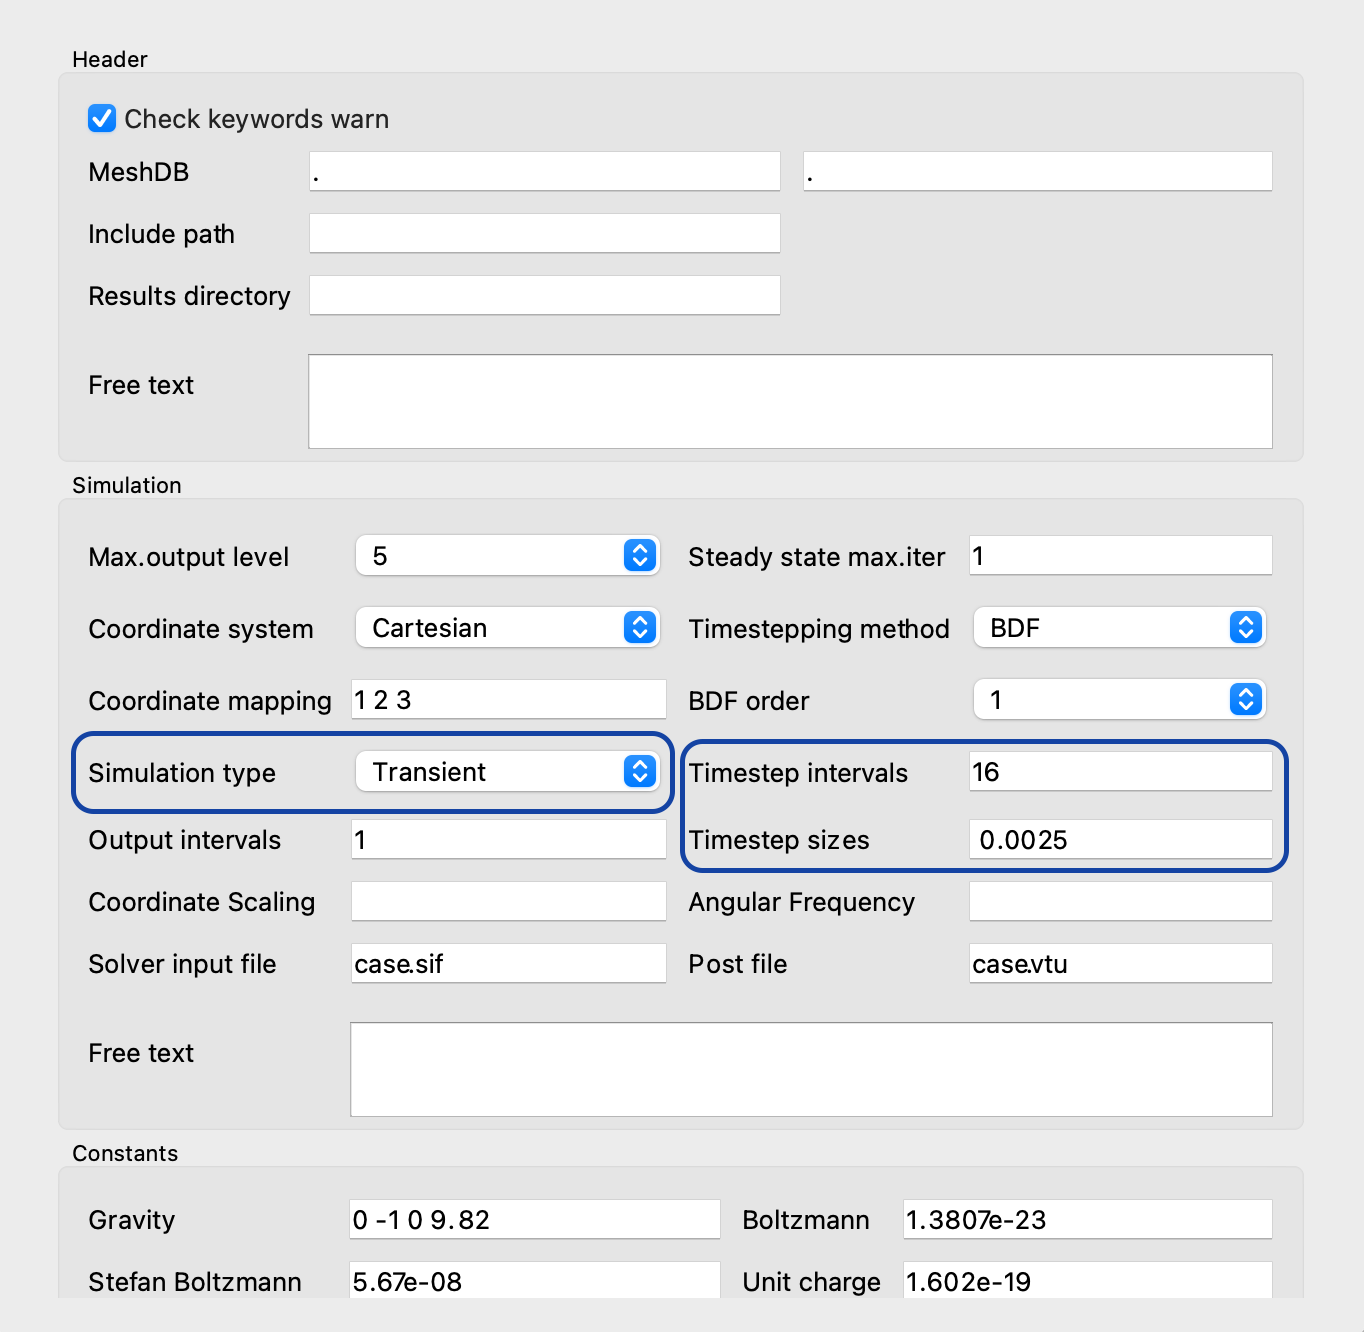
\includegraphics[width=0.6\textwidth]{figures/transient_setup.png}
\caption{Preferences Setup Window}\label{fg:time_setup}
\end{figure}  

\subsection*{Solution procedure}

At this point the mesh (Fig. \ref{fg:mesh}) has been loaded,  the model setup has been configured and the necessary menus have been added to the GUI.  We may now proceed to set up the physics of the TEAM Problem 7. 

\begin{figure}[H]
\centering
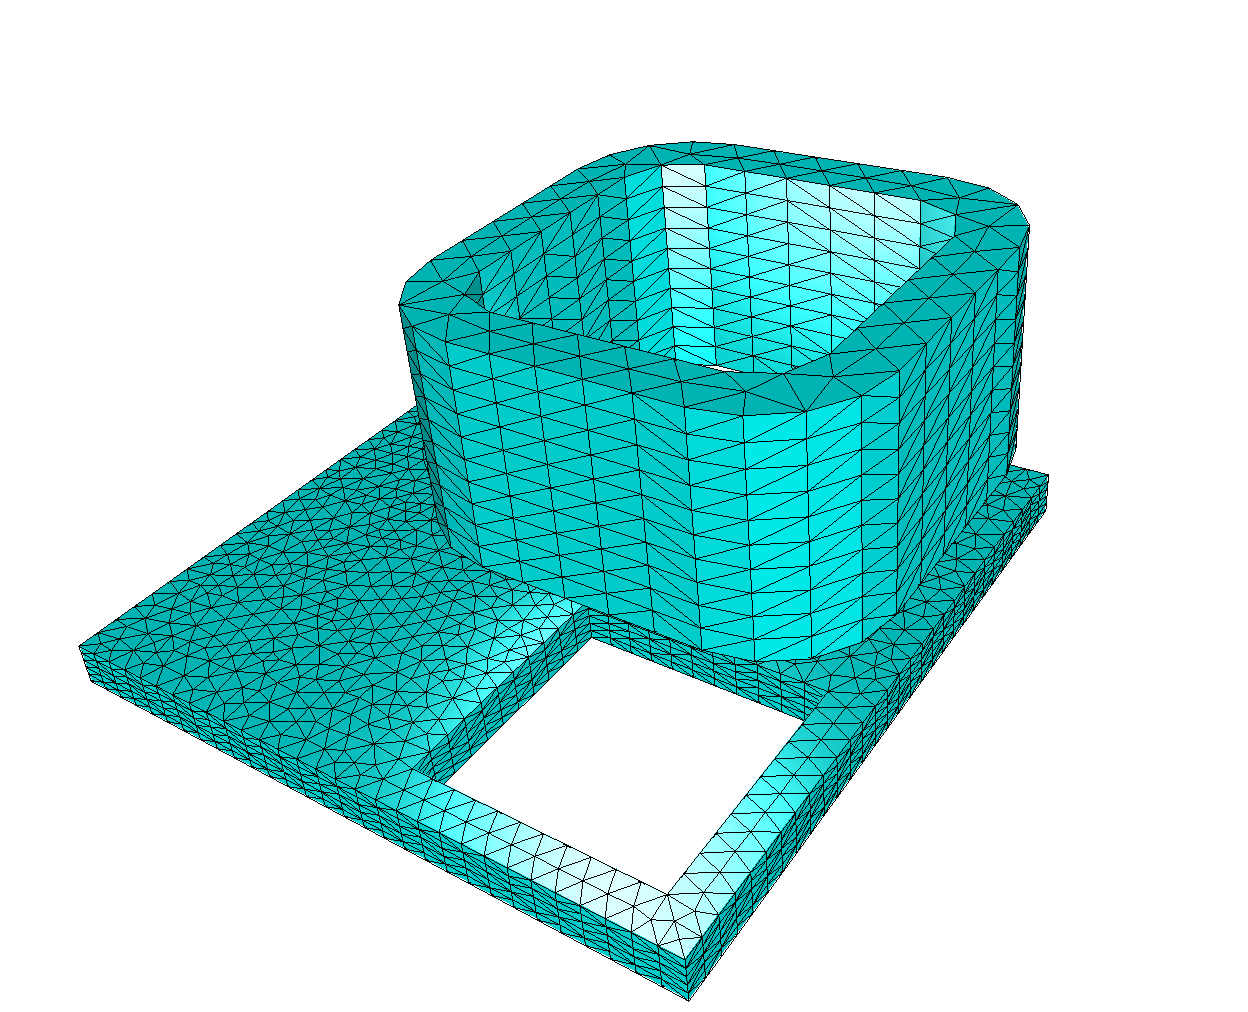
\includegraphics[width=0.7\textwidth]{figures/TEAM7_mesh.png}
\caption{TEAM 7 Mesh.}\label{fg:mesh}
\end{figure}



Let us configure the equations. Two sets of equations are needed in this problem. The first set of equations will apply to the Coil domain alone whereas the second set applies to the Plate and Air domain.  The reasoning behind it lies in the fact that we will solve the current direction before the simulation begins,  using it as a source in the magnetodynamics problem.

The coil equation are setup in the following manner
\ttbegin
Model
  Equation -> Add
     Name = Equation Coil
     Apply to Bodies = 1
     
     CoilSolver
         Active = on 
         Edit Solver Settings
             Solver specific options
                 Coil Closed=on
                 Desired Coil Current =  -2742
                 Normalize Coil Current=on
                 Coil Normal (3-vector) = 0 0 1
                 Narrow Interface=on
                 Fix Input Current Density=on
             General
                 Execute solver -> Before Simulation
             Apply
             
     MgDyn
         Active = on
         Edit Solver Settings
             Solver specific options
                 Use Elemental CoilCurrent=on
             Apply
         
     MgDynPost
         Active=on
         Edit Solver Settings
             Solver specific options
                 Specify fields to compute
                     Calculate Current Density=on
                 What kind of fields to compute
                     Discontinuous bodies=on
             General
                 Execute solver -> Before Saving
              Apply
    Add 
    OK
\ttend       


\clearpage
The configuration of the menus will appear also in any new equation added.  For this reason,  we only need activate the solvers needed and apply them to the respective bodies

\ttbegin
Model
  Equation -> Add
     Name = Equation Plate and Air
     Apply to Bodies = 1 2
     
     MgDyn
         Active = on
         
     MgDynPost
         Active=on
         
    Add 
    OK
\ttend  

 
Elmer contains an extensive material library however, for this exercise we will define some user defined material properties.  In this example we only need two materials: Air and Aluminium which are applied on. Due to the fact that the current is known a priori, the current density will be used as an external current source enabling the coil to be part of the non-conducting domain (Air).

\ttbegin
Model
  Material -> Add
      Name = Air
      Apply to Bodies = 1 3
      MgDyn
          Relative Permeability=1
    Update
    OK
\ttend


\ttbegin
Model
  Material -> Add
      Name = Aluminium
      Apply to Bodies = 2
      MgDyn
          Relative Permeability=1
          Electric Conductivity =3.526e7
    Update
    OK
\ttend

A Body Force represents the right-hand-side of a equation.  In this case we want to re-use the computed current density (by the Coil Solver) and use it in our MagnetoDynamics problem. By activating the \textit{ Use Elemental CoilCurrent=on} checkbox in the MgDyn solver menu, this action is performed.  However, since the current is sinusoidal, we will set up a feature that is found within the Body Force menu. 



\ttbegin
Model
  Body Force
    Name = External CoilCurrent Source
    Apply to Bodies = 1
    Current Density Multiplier= Variable "time"; Real LUA "cos(2*math.pi*50*tx[0])"
    Add 
    OK
\ttend    

Note that the frequency is 50Hz.  Hence  cos(2 $\pi$ f t), where f is the excitation frequency. 

\clearpage
\noindent Lastly,  at infinity the magnetic vector potential is set to zero

\ttbegin
Model
  BoundaryCondition -> Add
      Name = Infinity
      Apply to Boundaries = 6
      MgDyn
          AV \{e\} = 0.0
      
    Add
    Ok
\ttend   



For the execution ElmerSolver needs the mesh files and the command file.  We have now basically defined all the information for ElmerGUI to write the command file. After writing it we may also visually inspect the command file.
\ttbegin
Sif 
  Generate
  Edit -> Double check file has been generated accordingly to specs
\ttend

Before we can execute the solver save the the project. 

\ttbegin
File 
  Save Project
\ttend

After we have successfully saved the files we may start the solver.

\ttbegin
Run
  Start solver
\ttend

A convergence view automatically pops up showing relative changes of each iteration.

When there are some results to view we may start the postprocessor also.

\ttbegin
Run
  Start ParaView
\ttend

\clearpage
\subsection*{Results}

Note that this model's purpose is two fold.  First,  our goal is to setup a basic 3D eddy current problem.  Second,  we use this model for validation purposes.  

You may inspect the results with Paraview or with ElmerVTK.

\noindent The following image have been created using Paraview. 

\begin{figure}[ht!]
\centering
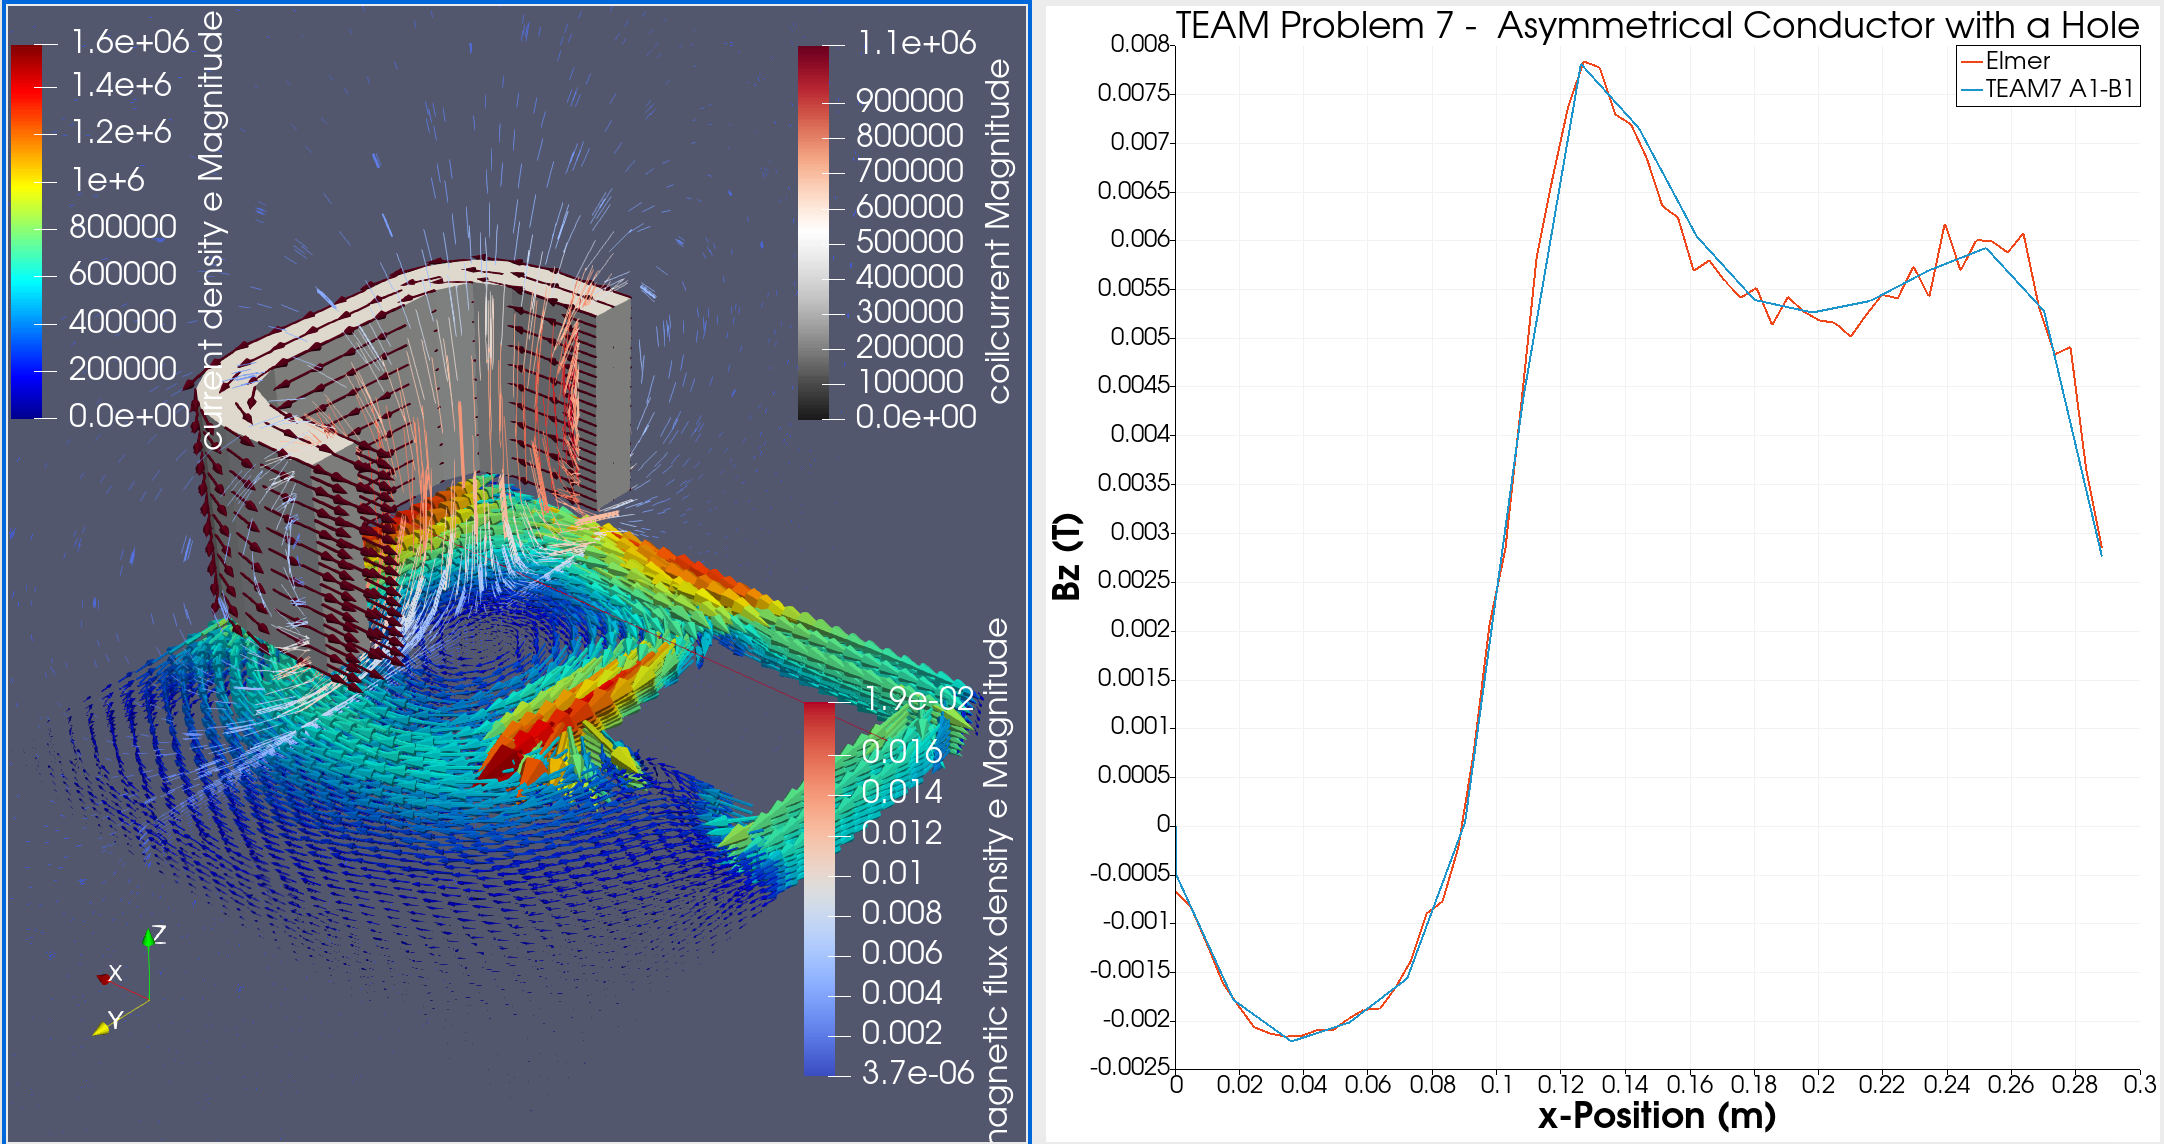
\includegraphics[width=\textwidth]{figures/results.png}
\caption{Postprocessing: Color map including induced currents on plate (Left),  Line Plot to validate Elmer's results against TEAM7's}\label{fg:results}
\end{figure} 



\hfill
